\section{Insertion Sort}
L'array viene virtualmente diviso in una parte ordinata e una non ordinata. I valori della parte non ordinata vengono prelevati e collocati nella posizione corretta della parte ordinata. \\

Caratteristiche dell'ordinamento per inserzione:
\begin{itemize}
    \item Questo algoritmo è uno dei più semplici e di semplice implementazione.
    \item Fondamentalmente, l'ordinamento per inserzione è efficiente per piccoli valori di dati
    \item L'ordinamento per inserzione è di natura adattativa, cioè è adatto a insiemi di dati già parzialmente ordinati.
\end{itemize}
Quello che sostanzialmente fa è esaminare gli elementi a coppie e ordinarli gradualmente per come si presentano.

\begin{center}
    \begin{tabular}{c}
        \\ 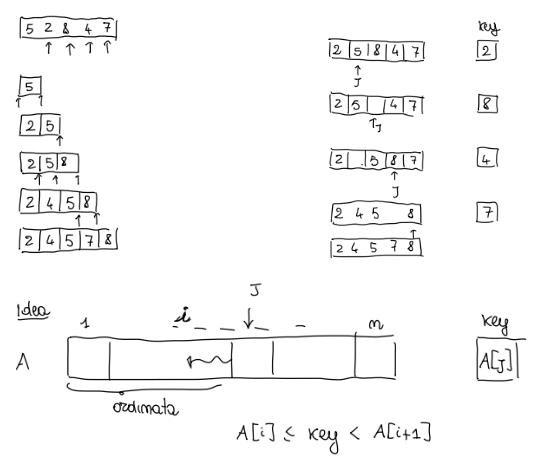
\includegraphics[width=0.5\textwidth]{image/InsertionSortExample.png} \\ \\
    \end{tabular}
\end{center}

\subsection{Pseudocodice}
\begin{mdframed}
\begin{lstlisting}[language=C]
INSERTION-SORT(A)
1   n = A.length
2   for j = 2 to n
3       key = A[j]
4       i = j - 1
5       while i > 0 and A[i] > key
6           A[i + 1] = A[i]
7           i = i - 1
8       A[i + 1] = key
\end{lstlisting}
\end{mdframed}

\subsection{Correttezza}
Definiamo i seguenti passi per $A$ da indice $1$ ad indice $j-1$
\paragraph{Inizializzazione:} $j=2, A[1,1]$ ordinato
\paragraph{Mantenimento:} inserisce $A[j]$ in $A[1 \; ... \; j-1]$ ordinato
\paragraph{Cancellazione:} $j=n+1$

\newpage